\documentclass[wide,a4paper,titlepage,12pt] {article}
\usepackage{polski}
\usepackage[utf8]{inputenc}
\usepackage{listings}
\usepackage{slashbox}
\usepackage[table]{xcolor}
\usepackage{graphicx,pdflscape}
\usepackage{placeins}


\title{Urządzenia peryferyjne}
\author{Tymon Tobolski (181037)\\ Jacek Wieczorek (181043)}

% Title page layout (fold)
\makeatletter
\renewcommand{\maketitle}{
\begin{titlepage}
  \begin{center}
    \vspace*{3cm}
    \LARGE \@title \par
    \vspace{2cm}
    \textit{\small Autor:}\par
    \normalsize \@author\par \normalsize
    \vspace{3cm}
    \textit{\small Prowadzący:}\par
    Dr inø. Jacek Mazurkiewicz \par
    \vspace{2cm}
    Wydział Elektroniki\\ III rok\\ Pn 8.15 - 11.00\par
    \vspace{4cm}
    \small \@date
  \end{center}
\end{titlepage}
}
\makeatother



\begin{document}
\maketitle

\section{Cel laboratorium}
\paragraph{}
Celem laboratorium było zapoznanie się z działaniem unipolarnego silnika krokowego
oraz sterowanie nim z komputera poprzez port szeregowy RS232.

\section{Działanie silnika krokowego}
\paragraph{}
Dwa silniki krokowe dostępne na laboratorium podłączone były do sterownika \textbf{MMusb245},
który zamieniał sygnal 8-bitowy pochodzący z portu szeregowago na analogowe sygnały sterujące uzwojeniami silników.

Silniki krokowe są obracane poprzez włączanie i wyłączanie uzwojeń silnika w odpowiedniej kolejności.
W opisanym programie zastosowane zostało sterowanie półkrokowe. Aby obrócić silnik należało wysłać poniższą sekwencje sygnałów:


\begin{center}
    \begin{tabular}{|c|c|c|c|}
    \hline
    0 1 0 1 \\
    \hline
    0 0 0 1 \\
    \hline
    1 0 0 1 \\
    \hline
    1 0 0 0 \\
    \hline
    1 0 1 0 \\
    \hline
    0 0 1 0 \\
    \hline
    0 1 1 0 \\
    \hline
    0 1 0 0 \\
    \hline
   \end{tabular}
\end{center}


\paragraph{}
Aby obrócić silnik w drugą stroną, należy wysłać podaną sekwencję w odwrotnej kolejności.

\paragraph{}
Sterownik pozwala na sterowanie dwoma silnikami krokowymi, pierwszym za pomocą młodszych 4 bitów wejścia, drugim za pomocą starszych 4 bitów.

\paragraph{}
Wartość pjedynczego skoku dla pierwszego silnika wynosiła 7.5$^\circ$, a dla drugiego 0.75$^\circ$.
Na podstawie tego wyliczana była ilość kroków potrzebna do obrotu silników o zadany kąt.


\section{Program}
\paragraph{}
Program wysyłający komendy do sterownika został napisane w języku C\# z wykorzystaniem biblioteki FTD2XX\_NET.
Pozwala on na sterowanie dwoma silnikami krokowymi na 2 sposoby. Pierwszy z nich to obrót silnika o zadaną ilość kroków w lewo lub w prawo.
Drugim sposobem sterowania jest obrót o zadany kąt, również w lewo lub w prawo.

\begin{figure}[htbp]
  \begin{center}
    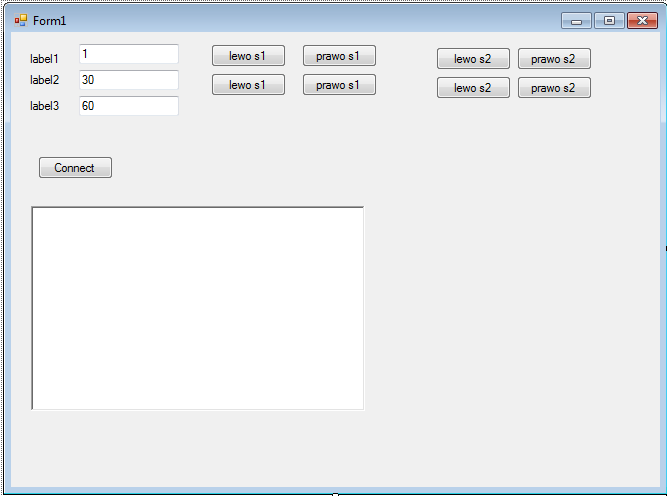
\includegraphics[width=\textwidth]{screen.png}
    \caption{Okno programu}
  \end{center}
\end{figure}


\section{Wnioski}
\paragraph{}
Program działa w pełni poprawnie z silnikami dostępnymi na laboratorium.
Największym problemem było dopasowanie odpowiedniej sekwencji pozwalającej na obrót silnikami.



\end{document}